\section{The 25~m and the 5~m model on the whole massifs}\label{app:dem}

Which elevation model should the crests come from? Section~\ref{sec:demres} ran the pipeline on four windows at 25~m and at 5~m and found the exponent on 0.1--1~km unchanged. Here we run both massifs whole, in four runs that change one thing at a time, and compare the counts, $\Hgeo$ and the box dimension. The report keeps the first run, and its numbers do not change. Numbers come from \code{compare\_dem.py}.

\subsection{Four runs}

Table~\ref{tab:cdruns} lists the runs. All of them use the same lengths in metres: the cross-section (\DrXsec~m), the bridged flat stretches (\DrBridge~m) and the pruned dead ends (\DrPrune~m) are fixed in metres and converted to cells of the run, as in Section~\ref{sec:demres}. The mountain area is drawn on 1~km cells from the model of each run.

\begin{table}[H]
\centering
\caption{Each run changes one thing from the one before. C1 is the run of the report.}
\label{tab:cdruns}
\small
\begin{tabular}{@{}l p{2.7cm} p{2.3cm} p{3.2cm} p{1.7cm} p{2cm}@{}}
\toprule
run & elevation model & rule for flats & footprint & routing & changes \\
\midrule
C1 & BD ALTI 25~m & flood & all BD ALTI tiles of the departments & in memory & \\
C2 & BD ALTI 25~m & order independent & all BD ALTI tiles of the departments & in memory & the rule for flats \\
C3 & RGE ALTI, every fifth cell & order independent & coverage of the 5~m model & in memory & the footprint \\
C4 & RGE ALTI 5~m & order independent & coverage of the 5~m model & by tiles & the resolution \\
\bottomrule
\end{tabular}
\end{table}

\paragraph{Rule for flats.} In C1 a cell of a flat drains to the cell that reached it in the priority flood, so its direction depends on the order in which the flood visits the cells. In C2 the cells of a flat drain by the gradients of Barnes, Lehman and Mulla~\cite{barnesflats}, which do not depend on that order.

\paragraph{Footprint.} The 25~m tiles of the departments hold elevations beyond the departments and beyond the French border, and the 5~m mosaic stops at the departments. C3 reads the 5~m model at every fifth cell, on the grid of BD ALTI, and has no data where the 5~m model has none. Where both models exist they are equal, cell by cell. So C2 and C3 differ by the footprint alone.

\paragraph{Routing.} C1 to C3 route the water in memory. The 5~m model of a massif does not fit in memory, so C4 routes it by tiles (\code{tiled.py}): depression filling by the priority flood of Barnes~\cite{barnesfill}, the flats of Barnes, Lehman and Mulla, and the drainage area by the accumulation of Barnes~\cite{barnesacc}; a flat that crosses tiles is gathered whole. At 25~m the routing by tiles gives the rasters of the routing in memory bit for bit on both massifs (\code{check\_tiled.py}; only the numbers of the links differ). So C3 and C4 differ by the resolution alone.

\subsection{Counts}

Table~\ref{tab:cdcounts} gives the counts. The flat rule changes the crest length by \CdAlpsLenPctRule\% in the Alps and \CdPyrLenPctRule\% in the Pyrenees. The footprint changes the most: the mountain area shrinks by \CdAlpsAreaPctFoot\% and \CdPyrAreaPctFoot\%, the crest length by \CdAlpsLenPctFoot\% and \CdPyrLenPctFoot\%, and the density of crest length by \CdAlpsDensPctFoot\% and \CdPyrDensPctFoot\%. The resolution adds crest: the length grows by \CdAlpsLenPctRes\% and \CdPyrLenPctRes\%, and the number of curves by \CdAlpsCurvesPctRes\% and \CdPyrCurvesPctRes\%. The medians of curves and paths move little. The longest path of the Alps is \CdAlpsLongPathThree~km in C3 and \CdAlpsLongPathFour~km in C4, and the paths of 40~km or more fall from \CdAlpsPathsFortyThree{} to \CdAlpsPathsFortyFour{} in \CdAlpsTreesFortyThree{} and \CdAlpsTreesFortyFour{} trees. We did not look for the cause.

\begin{table}[H]
\centering
\caption{The footprint changes the counts most, the resolution adds crest, and the flat rule changes almost nothing. Crest curves are the curves before the joins; lengths in km. A path of 40~km or more reaches a lag of 10~km, since lags stop at a quarter of the path.}
\label{tab:cdcounts}
\footnotesize
\setlength{\tabcolsep}{3.5pt}
\begin{tabular}{lrrrrrrrr}
\toprule
 & \multicolumn{4}{c}{Alps} & \multicolumn{4}{c}{Pyrenees} \\
\cmidrule(lr){2-5}\cmidrule(lr){6-9}
 & C1 & C2 & C3 & C4 & C1 & C2 & C3 & C4 \\
\midrule
\tablerows{generated/compare_dem_counts}
\bottomrule
\end{tabular}
\end{table}

\subsection{Exponents}

Table~\ref{tab:cdh} gives $\Hgeo$ of the paths and of the single curves on the windows of Table~\ref{tab:hgeo}. Table~\ref{tab:cdd} gives the box and the divider dimension of the paths on the windows of Section~\ref{sec:dimension}, and the box dimension of the network of all the curves on the small and the large boxes of Rak et al.~\cite{rak}. The intervals are 95\% bootstrap intervals over whole trees, as in Table~\ref{tab:hgeo}.

\begin{table}[H]
\centering
\caption{On the windows below 10~km the intervals of the four runs overlap, with one exception, and beyond 10~km the estimates part. $\Hgeo$ of the paths and of the single curves of each run, with 95\% intervals under the estimates. The exception is the window 0.1--1~km of the Pyrenees, where C2 and C4 do not overlap. The window beyond 10~km has no curves, and the window 1--10~km of the curves mixes populations (Appendix~\ref{app:limits}).}
\label{tab:cdh}
\footnotesize
\setlength{\tabcolsep}{4pt}
\begin{tabular}{lrrrr}
\toprule
 & C1 & C2 & C3 & C4 \\
\midrule
\tablerows{generated/compare_dem_hgeo}
\bottomrule
\end{tabular}
\end{table}

\begin{table}[H]
\centering
\caption{The box dimension of the paths changes by at most \CdMaxDeltaDAny{} between two runs that share a class of curves. Box and divider dimension of the crest paths on the windows of Section~\ref{sec:dimension}, with 95\% intervals under the estimates, and box dimension of the network of the curves. In the Pyrenees the 5~m footprint has \CdPyrGroupsThirtyTwoThree{} trees (C3) and \CdPyrGroupsThirtyTwoFour{} trees (C4) with a path of 32~km or more, fewer than \DmMinGroups, so the windows from 0.1~km and 1--10~km use the class of 16~km in C3 and C4 and that of 32~km in C1 and C2: they cannot be compared across the footprint.}
\label{tab:cdd}
\footnotesize
\setlength{\tabcolsep}{4pt}
\begin{tabular}{lrrrr}
\toprule
 & C1 & C2 & C3 & C4 \\
\midrule
\tablerows{generated/compare_dem_dimension}
\bottomrule
\end{tabular}
\end{table}

\paragraph{Rule for flats.} The rule changes no exponent. On the windows below 10~km $\Hgeo$ of the paths changes by at most \CdMaxDeltaHRule, the box dimension by at most \CdMaxDeltaDRule, and every interval of $\Hgeo$ holds the estimate of the other run. Beyond 10~km $\Hgeo$ changes by \CdAlpsDeltaHLongRule{} in the Alps and \CdPyrDeltaHLongRule{} in the Pyrenees.

\paragraph{Footprint.} The window 0.1--1~km changes by \CdAlpsDeltaHShortFoot{} in the Alps and \CdPyrDeltaHShortFoot{} in the Pyrenees, and the other two windows below 10~km by at most \CdMaxDeltaHFoot, inside the intervals. The box dimension changes by at most \CdMaxDeltaDFoot{} where the class is the same. Beyond 10~km $\Hgeo$ changes by \CdAlpsDeltaHLongFoot{} in the Alps and \CdPyrDeltaHLongFoot{} in the Pyrenees. This window rests on the paths of 40~km or more, and the 5~m footprint has \CdAlpsPathsFortyThree{} of them in the Alps against \CdAlpsPathsFortyTwo{}, and \CdPyrPathsFortyThree{} in the Pyrenees against \CdPyrPathsFortyTwo{} (Table~\ref{tab:cdcounts}). The dimension of the network on the large boxes changes by \CdAlpsDNetLargeDeltaFoot{} and \CdPyrDNetLargeDeltaFoot, and on the small boxes by \CdAlpsDNetSmallDeltaFoot{} and \CdPyrDNetSmallDeltaFoot.

\paragraph{Resolution.} Below 10~km $\Hgeo$ changes by at most \CdMaxDeltaHRes, on the window from 0.1~km of the Alps (\CdAlpsDeltaHFromRes), and the intervals of C3 and C4 overlap on every window below 10~km. Between C2 and C4 the window 0.1--1~km of the Pyrenees changes by \CdPyrDeltaHShortTwoFour, and there the intervals do not overlap. The window 0.1--1~km changes by \CdAlpsDeltaHShortRes{} in the Alps and \CdPyrDeltaHShortRes{} in the Pyrenees. The box dimension of the paths changes by at most \CdMaxDeltaDRes. The network gains \CdAlpsDNetSmallDeltaRes{} (Alps) and \CdPyrDNetSmallDeltaRes{} (Pyrenees) on the small boxes and changes by \CdAlpsDNetLargeDeltaRes{} and \CdPyrDNetLargeDeltaRes{} on the large ones. Beyond 10~km $\Hgeo$ changes by \CdAlpsDeltaHLongRes{} in the Alps and \CdPyrDeltaHLongRes{} in the Pyrenees. The single curves go from \CdAlpsHCurvesFromOne{} in C1 to \CdAlpsHCurvesFromFour{} in C4 in the Alps and from \CdPyrHCurvesFromOne{} to \CdPyrHCurvesFromFour{} in the Pyrenees on the window from 0.1~km.

\begin{figure}[H]
\centering
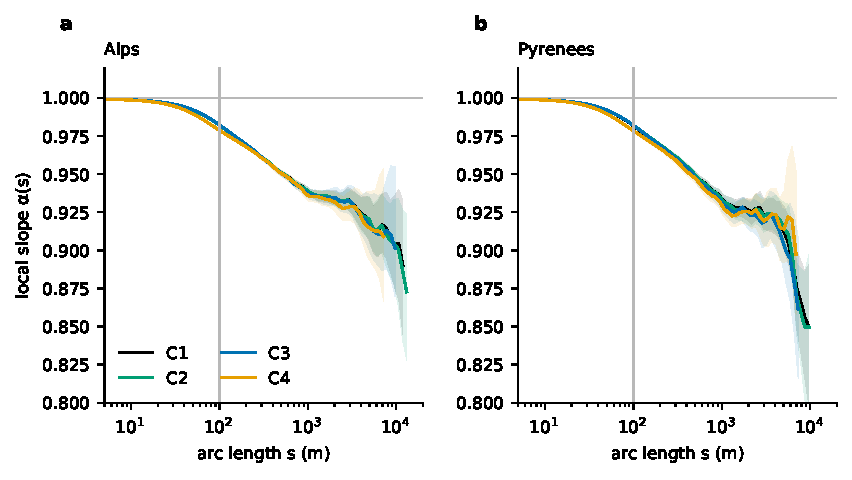
\includegraphics[width=\textwidth]{figures/compare_dem_alpha.pdf}
\caption{The local slope of the paths is the same in the four runs up to 5~km. $\alpha(s)$ of the paths of C1 to C4 with 95\% bands over trees, for the lags that at least \CdMinRows{} paths reach and whose band is at most 0.1 wide. Grey line: 100~m. Largest difference to C1: \CdAlphaSpreadShort{} on 0.1--1~km, \CdAlphaSpreadMid{} on 1--5~km and \CdAlphaSpreadLong{} on 5--10~km. \textbf{a}~Alps. \textbf{b}~Pyrenees.}
\label{fig:cdalpha}
\end{figure}

Figure~\ref{fig:cdalpha} shows the same on every lag. The four curves follow each other up to 5~km. Between 5 and 10~km they part, where the bands are wide.

\subsection{Where the crests differ}

Figure~\ref{fig:cdzoom} draws C3 and C4 on the 5~m hillshade, in the \CdZoomKm~km square of each massif where the two runs differ most: the square with the most points that only one run has, among the squares where both runs have at least \CdMinPoints{} points. A point of one run belongs to it alone if the other run has no point within \CdTolM~m. Over the whole massif \CdAlpsOnlyThree\% of the points of C3 and \CdAlpsOnlyFour\% of those of C4 belong to one run alone in the Alps, and \CdPyrOnlyThree\% and \CdPyrOnlyFour\% in the Pyrenees. Inside the two squares the shares are \CdAlpsSqOnlyThree\% and \CdAlpsSqOnlyFour\% in the Alps and \CdPyrSqOnlyThree\% and \CdPyrSqOnlyFour\% in the Pyrenees: the squares are the most different places, and the average place differs less.

\begin{figure}[H]
\centering
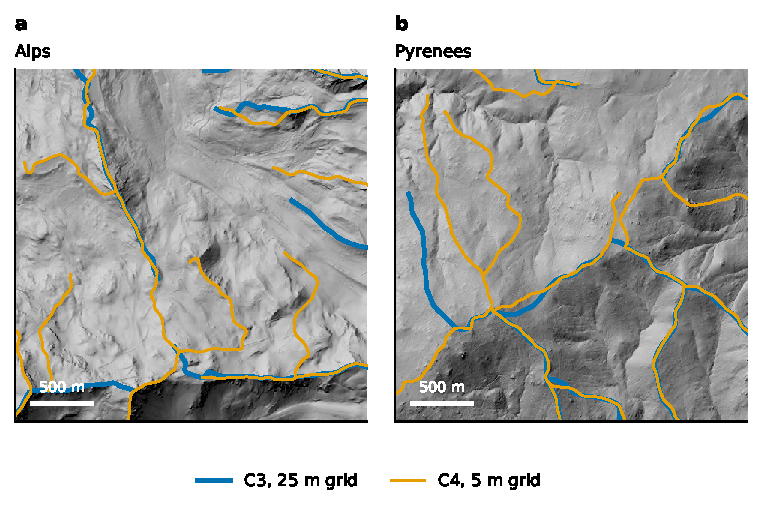
\includegraphics[width=\textwidth]{figures/compare_dem_zoom.pdf}
\caption{Each run has crest that the other lacks. Crest curves of C3 (25~m grid, thick) and C4 (5~m grid, thin) on the hillshade of the 5~m model, in a \CdZoomKm~km square where they differ most. \textbf{a}~Alps. \textbf{b}~Pyrenees.}
\label{fig:cdzoom}
\end{figure}

\paragraph{What we keep.} Which model? On the windows below 10~km the 25~m model is enough. The window 0.1--1~km is \CdAlpsHPathsShortOne{} in C1 and \CdAlpsHPathsShortFour{} in C4 in the Alps, and \CdPyrHPathsShortOne{} and \CdPyrHPathsShortFour{} in the Pyrenees. No step changes $\Hgeo$ of the paths on the three windows below 10~km by more than \CdMaxDeltaHAny, nor the box dimension by more than \CdMaxDeltaDAny. Only the window 0.1--1~km of the Pyrenees separates two runs beyond their intervals, C2 and C4, by \CdPyrDeltaHShortTwoFour. The 5~m model adds \CdAlpsLenPctRes\% and \CdPyrLenPctRes\% of crest length. Its footprint is smaller by \CdAlpsAreaPctFoot\% and \CdPyrAreaPctFoot\% of the mountain area. So the report keeps C1.

The answer is weak beyond 10~km. There $\Hgeo$ of the paths goes from \CdAlpsHPathsLongOne{} (C1) to \CdAlpsHPathsLongFour{} (C4) in the Alps and from \CdPyrHPathsLongOne{} to \CdPyrHPathsLongFour{} in the Pyrenees, with wide intervals, because the window rests on \CdAlpsTreesFortyOne{} trees in the Alps and \CdPyrTreesFortyOne{} in the Pyrenees in C1, and on \CdAlpsTreesFortyFour{} and \CdPyrTreesFortyFour{} in C4. In the Pyrenees the footprint moves this window more than the resolution, in the Alps the resolution moves it more. This window needs more trees, and the smaller footprint of the 5~m model gives fewer. The box dimension of the Pyrenees on the windows from 0.1~km and 1--10~km depends on the class of curves, which the footprint changes, so only the window 0.1--1~km is comparable across all four runs there.
